% The contents of this file is 
% Copyright (c) 2009-  Charles R. Severance, All Righs Reserved

\chapter{Visualizando dados}
%\chapter{Visualizing data}

Até agora, nós aprendemos a linguagem Python, como utilizá-la,
para trabalhar com redes e banco de dados para manipular dados.
%So far we have been learning the Python language and then 
%learning how to use Python, the network, and databases 
%to manipulate data.

Neste capítulo, serão apresentadas três aplicações completas
que utilizarão todos estes conceitos para gerenciar e visualizar
dados. Você pode utilizar estas aplicações como exemplo de código
que podem ajudar na solução de problemas reais. 
%In this chapter, we take a look at three 
%complete applications that bring all of these things together
%to manage and visualize data.  You  might use these applications 
%as sample code to help get you started in solving a
%real-world problem.

Cada uma das aplicações é um arquivo ZIP que você pode fazer
download, extrair para o seu computador e executar.
%Each of the applications is a ZIP file that you can download
%and extract onto your computer and execute.

\section{Construindo um mapa no Google a partir de dados geocodificados}
\index{Google!map}
\index{Visualização!mapas}
%\section{Building a Google map from geocoded data}
%\index{Google!map}
%\index{Visualization!map}

Neste projeto, nós utilizaremos a API de geocodificação do
Google para obter algumas localizações geográficas informadas
pelos usuários de nomes de universidades e colocar os dados
em um mapa no Google.
%In this project, we are using the Google geocoding API
%to clean up some user-entered geographic locations of 
%university names and then placing the data on a Google
%map.  

\beforefig
\centerline{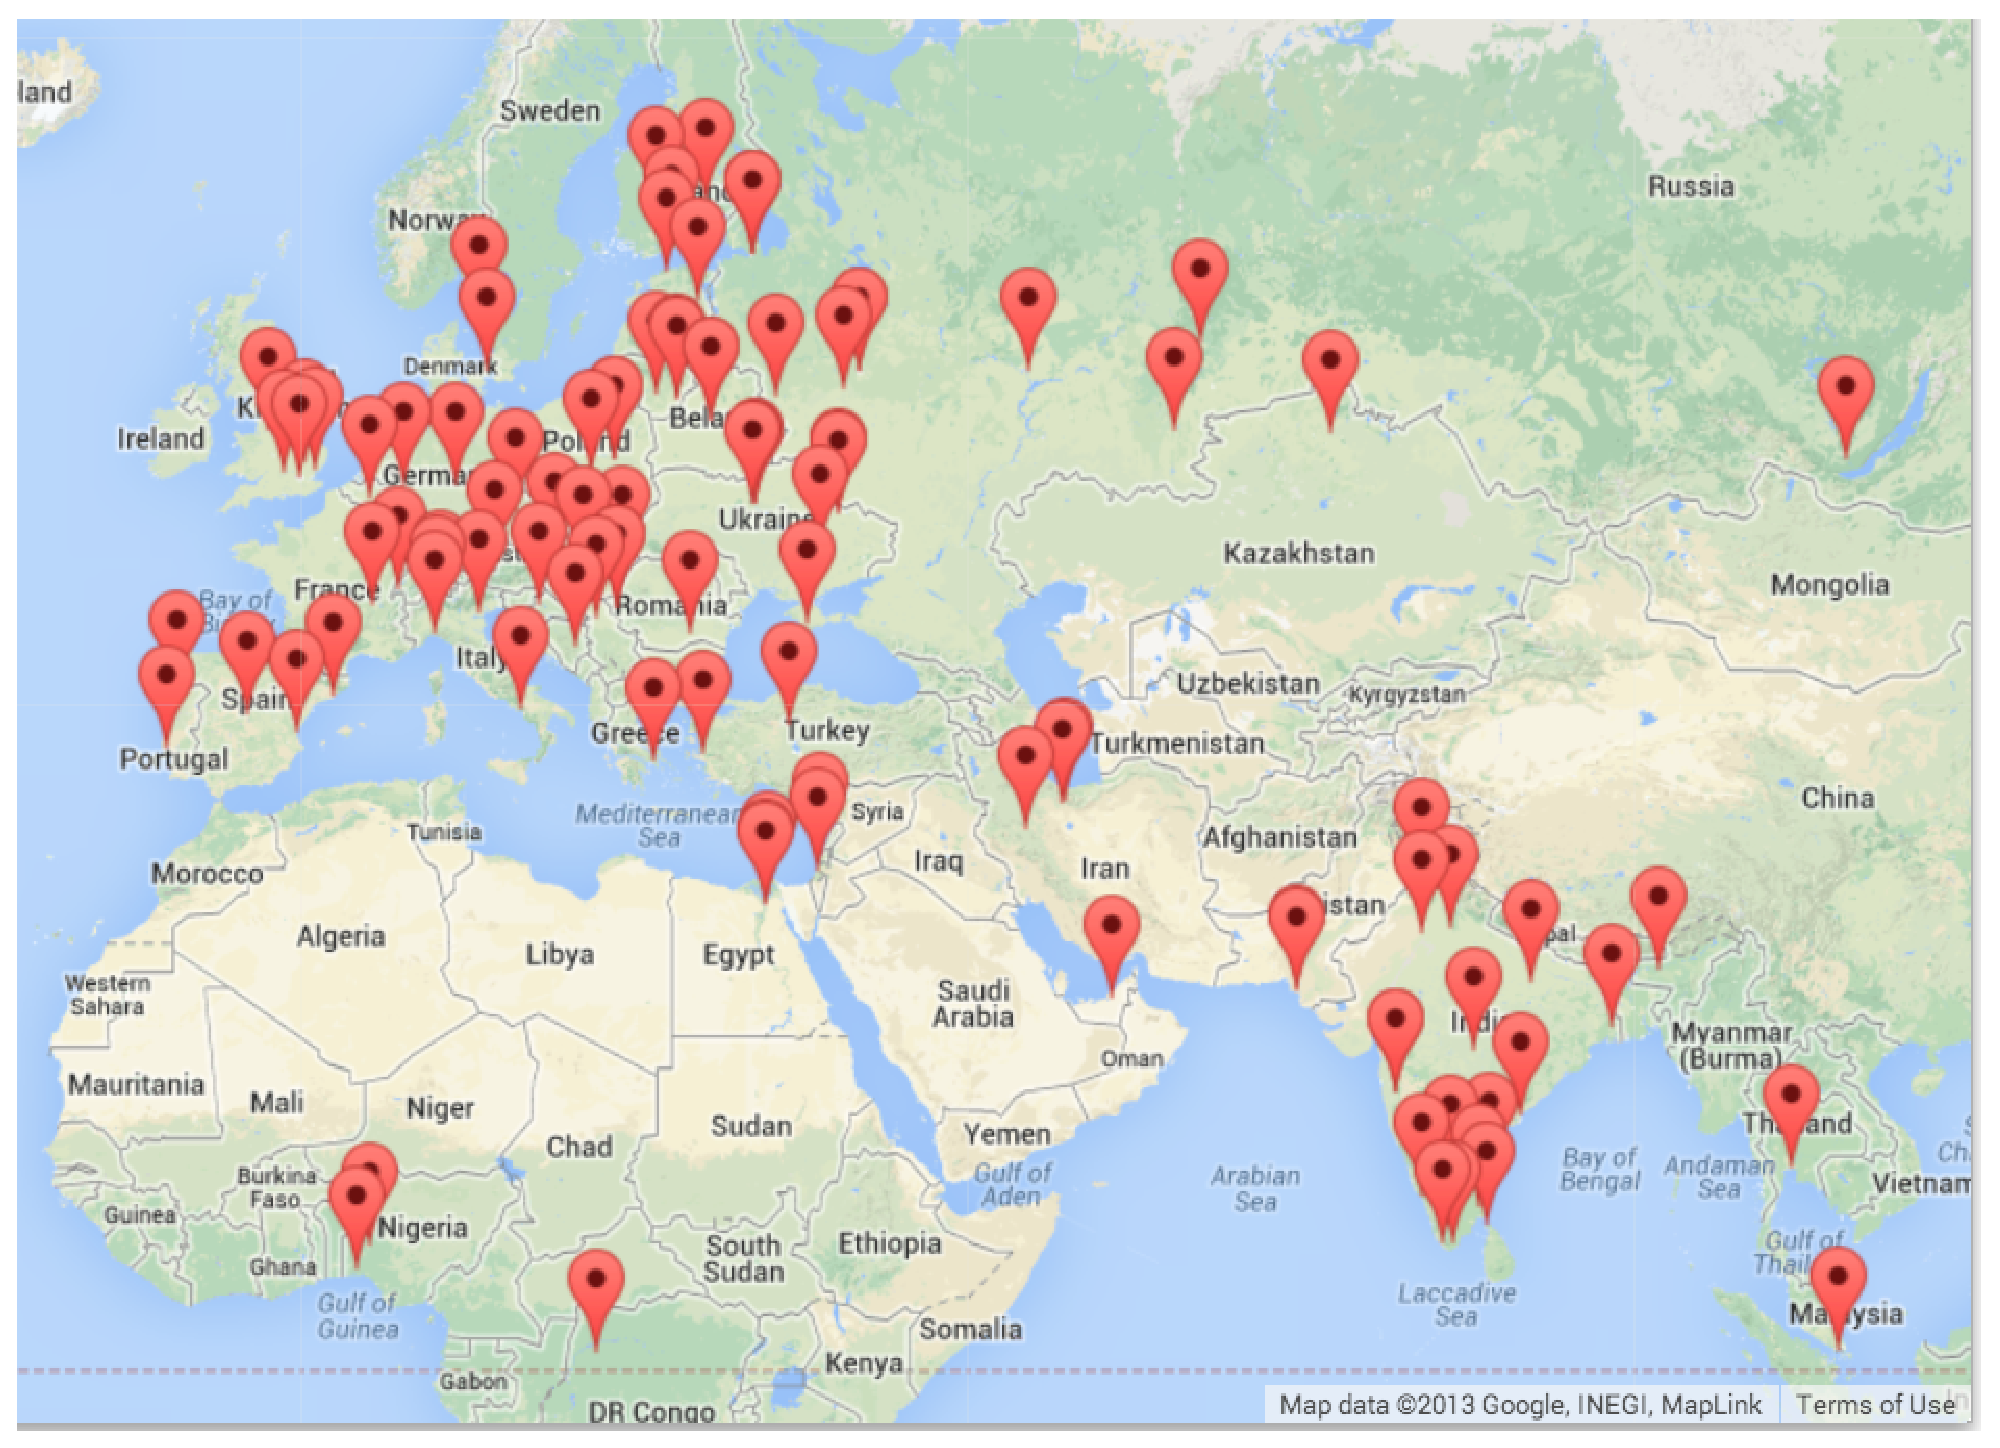
\includegraphics[height=2.25in]{figs2/google-map.eps}}
\afterfig
%\beforefig
%\centerline{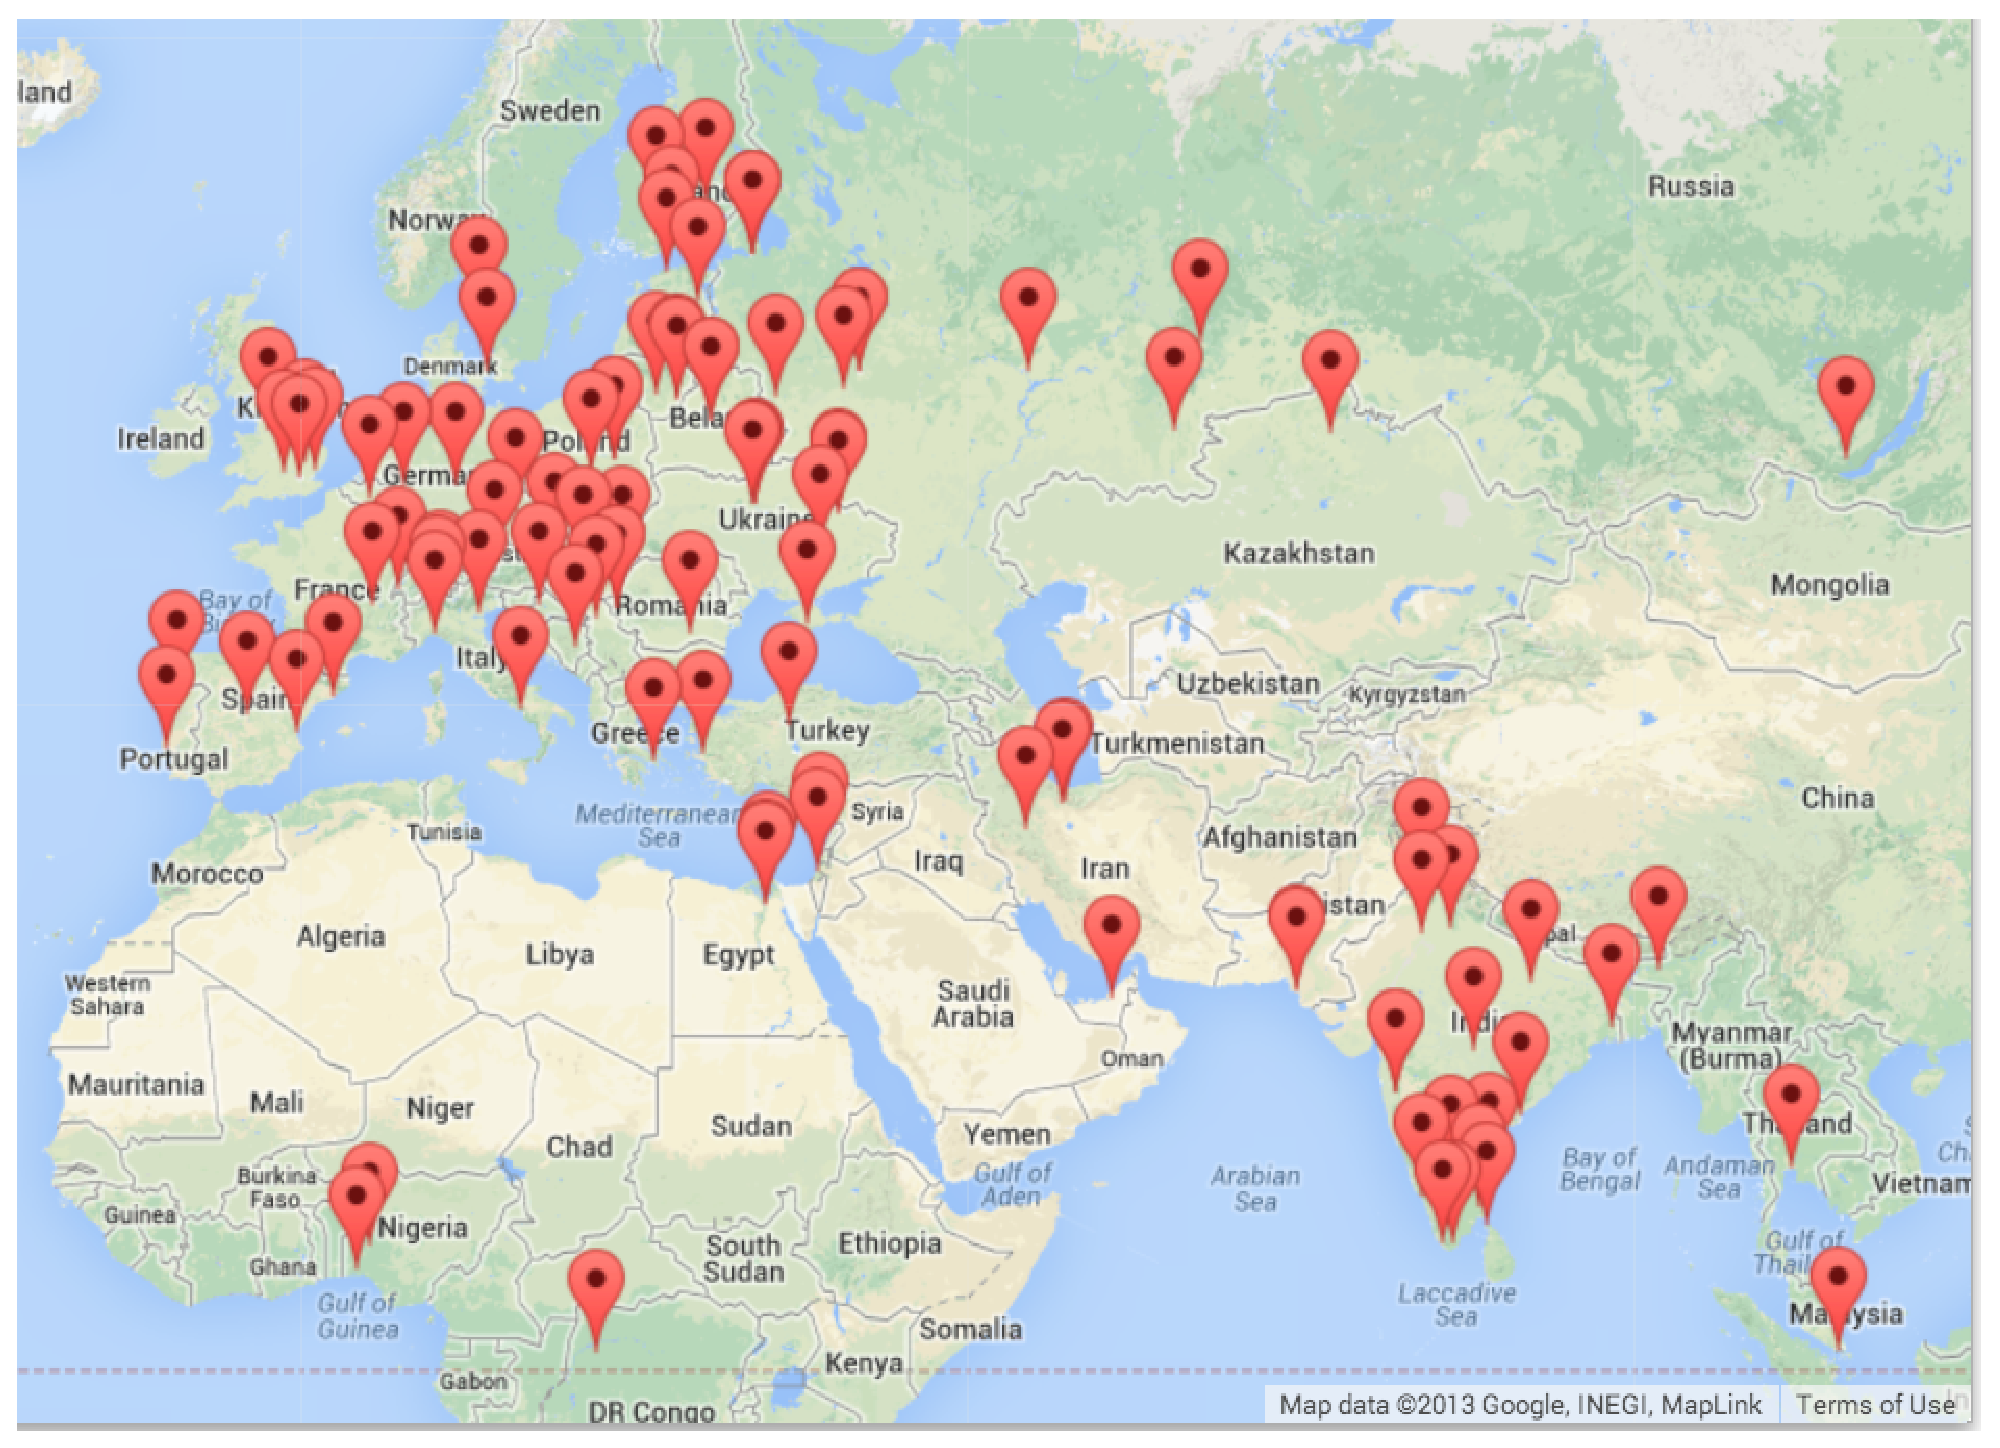
\includegraphics[height=2.25in]{figs2/google-map.eps}}
%\afterfig

Para iniciar, faça o download da aplicação em:
%To get started, download the application from:

\url{www.py4inf.com/code/geodata.zip}

O primeiro problema a ser resolvido é que a API gratuita de 
geocodificação do Google limita o número de requisições por dia.
Se você tiver muitos dados, você pode precisar parar e reiniciar
o processo de busca muitas vezes. Nós podemos quebrar o problema
em duas fases.
%The first problem to solve is that the free Google geocoding
%API is rate-limited to a certain number of requests per day.  If you have
%a lot of data, you might need to stop and restart the lookup
%process several times.  So we break the problem into two
%phases.  

\index{cache}
Na primeira fase nós faremos uma ``'pesquisa'' nos dados do arquivo
{\bf where.data} e então ler uma linha por vez, retornando a informação
geocodificada do Google e armazenar em um banco de dados {\bf geodata.sqlite}.
Antes de efetuar a pesquisa no Google, utilizando a API, para cada localização
informada pelo usuário, nós vamos checar para ver se já existe este dado
para a localização informada. O banco de dados está funcionando como um
``cache'' local dos nossos dados de localização para ter certeza que nunca
buscaremos no Google duas vezes pelo mesmo dado.
%\index{cache}
%In the first phase we take our input ``survey'' data in the file
%{\bf where.data} and read it one line at a time, and retrieve the
%geocoded information from Google and store it 
%in a database {\bf geodata.sqlite}.
%Before we use the geocoding API for each user-entered location, 
%we simply check to see if we already have the data for that 
%particular line of input.  The database is functioning as a 
%local ``cache'' of our geocoding data to make sure we never ask 
%Google for the same data twice.

Você pode reiniciar o processo a qualquer hora deletando o arquivo 
{\bf geodata.sqlite}.
%You can restart the process at any time by removing the file
%{\bf geodata.sqlite}.

Execute o programa {\bf geoload.py}. Este programa fará a leitura das linhas
do arquivo {\bf where.data} e para cada linha checar se o dado já existe no
banco de dados. Se nós não tivermos o dado para a localização, será utilizada
a API para retornar o dado e armazená-lo no banco de dados.  
%Run the {\bf geoload.py} program.   This program will read the input
%lines in {\bf where.data} and for each line check to see if it is already
%in the database.  If we don't have the data for the location, it will
%call the geocoding API to retrieve the data and store it in 
%the database.

Aqui está uma simples execução após a coleta de alguns dados no
banco de dados:
%Here is a sample run after there is already some data in the 
%database:

\beforeverb
\begin{verbatim}
Found in database  Northeastern University
Found in database  University of Hong Kong, ...
Found in database  Technion
Found in database  Viswakarma Institute, Pune, India
Found in database  UMD
Found in database  Tufts University

Resolving Monash University
Retrieving http://maps.googleapis.com/maps/api/
    geocode/json?sensor=false&address=Monash+University
Retrieved 2063 characters {    "results" : [  
{u'status': u'OK', u'results': ... }

Resolving Kokshetau Institute of Economics and Management
Retrieving http://maps.googleapis.com/maps/api/
    geocode/json?sensor=false&address=Kokshetau+Inst ...
Retrieved 1749 characters {    "results" : [  
{u'status': u'OK', u'results': ... }
...
\end{verbatim}
\afterverb
%

As primeiras cinco execuções já estão no banco de dados e então serão
ignoradas. O programa encontra o ponto onde parou e então continua
o trabalho recuperando novas informações.
%The first five locations are already in the database and so they 
%are skipped.  The program scans to the point where it finds new
%locations and starts retrieving them.

O programa {\bf geoload.py} pode ser parado a qualquer hora, e há um
contador que você pode utilizar para limitar o número de chamadas para a
API de geocodificação a cada execução. Dado o arquivo {\bf where.data}, que
possui algumas centenas de itens, você não consegue ultrapassar o limite diário,
mas pode fazer várias execuções em vários dias diferentes para ir pegando
aos poucos todos os dados que você precisa.
%The {\bf geoload.py} program can be stopped at any time, and there is a counter 
%that you can use to limit the number of calls to the geocoding
%API for each run.  Given that the {\bf where.data} only has a few hundred
%data items, you should not run into the daily rate limit, but if you 
%had more data it might take several runs over several days to 
%get your database to have all of the geocoded data for your input.

Uma vez que você tiver alguns dados carregados em {\bf geodata.sqlite},
você pode visualizar os dados utilizando o programa {\bf geodump.py}.
Este programa lê o banco de dados e escreve no arquivo {\bf where.js}
com a localização de latitude e longitude em um formato de código 
JavaScript.
%Once you have some data loaded into {\bf geodata.sqlite}, you can 
%visualize the data using the {\bf geodump.py} program.  This
%program reads the database and writes the file {\bf where.js}
%with the location, latitude, and longitude in the form of
%executable JavaScript code.   

Segue uma execução do programa {\bf geodump.py}:
%A run of the {\bf geodump.py} program is as follows:

\beforeverb
\begin{verbatim}
Northeastern University, ... Boston, MA 02115, USA 42.3396998 -71.08975
Bradley University, 1501 ... Peoria, IL 61625, USA 40.6963857 -89.6160811
...
Technion, Viazman 87, Kesalsaba, 32000, Israel 32.7775 35.0216667
Monash University Clayton ... VIC 3800, Australia -37.9152113 145.134682
Kokshetau, Kazakhstan 53.2833333 69.3833333
...
12 records written to where.js
Open where.html to view the data in a browser
\end{verbatim}
\afterverb
%

O arquivo {\bf where.html} consiste de um HTML e um JavaScript para visualizar
um mapa Google. Ele lê os dados mais recentes em {\bf where.js} para pegar
os dados a serem visualizados. Aqui está um formato do arquivo {\bf where.js}.
%The file {\bf where.html} consists of HTML and JavaScript to visualize 
%a Google map.  It reads the most recent data in {\bf where.js} to get 
%the data to be visualized.  Here is the format of the {\bf where.js} file:

\beforeverb
\begin{verbatim}
myData = [
[42.3396998,-71.08975, 'Northeastern Uni ... Boston, MA 02115'],
[40.6963857,-89.6160811, 'Bradley University, ... Peoria, IL 61625, USA'],
[32.7775,35.0216667, 'Technion, Viazman 87, Kesalsaba, 32000, Israel'],
   ...
];
\end{verbatim}
\afterverb
%

Esta é uma variável JavaScript que contém uma lista de listas.
A sintaxe para representação de listas em JavaScript é muito similar
ao Python, sendo assim, deve ser familiar para você também.
%This is a JavaScript variable that contains a list of lists.  
%The syntax for JavaScript list constants is very similar to 
%Python, so the syntax should be familiar to you.

Simplemente abra o arquivo {\bf where.html} em um browser para ver as
localizações. Você pode passar o mouse por cima de cada um dos pontos 
do mapa para encontrar a localização que a API de geocodificação retornou
para uma entrada do usuário. Se você não puder ver qualquer dado quando
abrir o arquivo {\bf where.html}, você pode querer checar o console do
desenvolvedor (JavaScript) de seu browser e ver se envcontra algum erro.
%Simply open {\bf where.html} in a browser to see the locations.  You 
%can hover over each map pin to find the location that the 
%geocoding API returned for the user-entered input.  If you 
%cannot see any data when you open the {\bf where.html} file, you might 
%want to check the JavaScript or developer console for your browser.

\section{Visualizando redes e interconexões}
\index{Google!page rank}
\index{Visualização!redes}
\index{Visualização!page rank}
%\section{Visualizing networks and interconnections}
%\index{Google!page rank}
%\index{Visualization!networks}
%\index{Visualization!page rank}

Nesta aplicação, vamos realizar algumas das funções de um motor de busca.
Nós primeiramente vamos extrair um pequeno pedaço da web e rodar
uma versão simplificada do algoritmo de page rank do Google para determinar
quais páginas estão altamente conectadas, e então visualizar o page rank
e a conectividade de nosso pequeno pedaço da web.
Utilizaremos a biblioteca de visualização JavaScript D3 \url{http://d3js.org/}
para produzir a saída da visualização.
%In this application, we will perform some of the functions of a search
%engine.   We will first spider a small subset of the web and run
%a simplified version of the Google page rank algorithm to
%determine which pages are most highly connected, and then visualize
%the page rank and connectivity of our small corner of the web.
%We will use the D3 JavaScript visualization library 
%\url{http://d3js.org/} to produce the visualization output.

Você pode fazer download e extrair esta aplicação de:
%You can download and extract this application from:

\url{www.py4inf.com/code/pagerank.zip}

\beforefig
\centerline{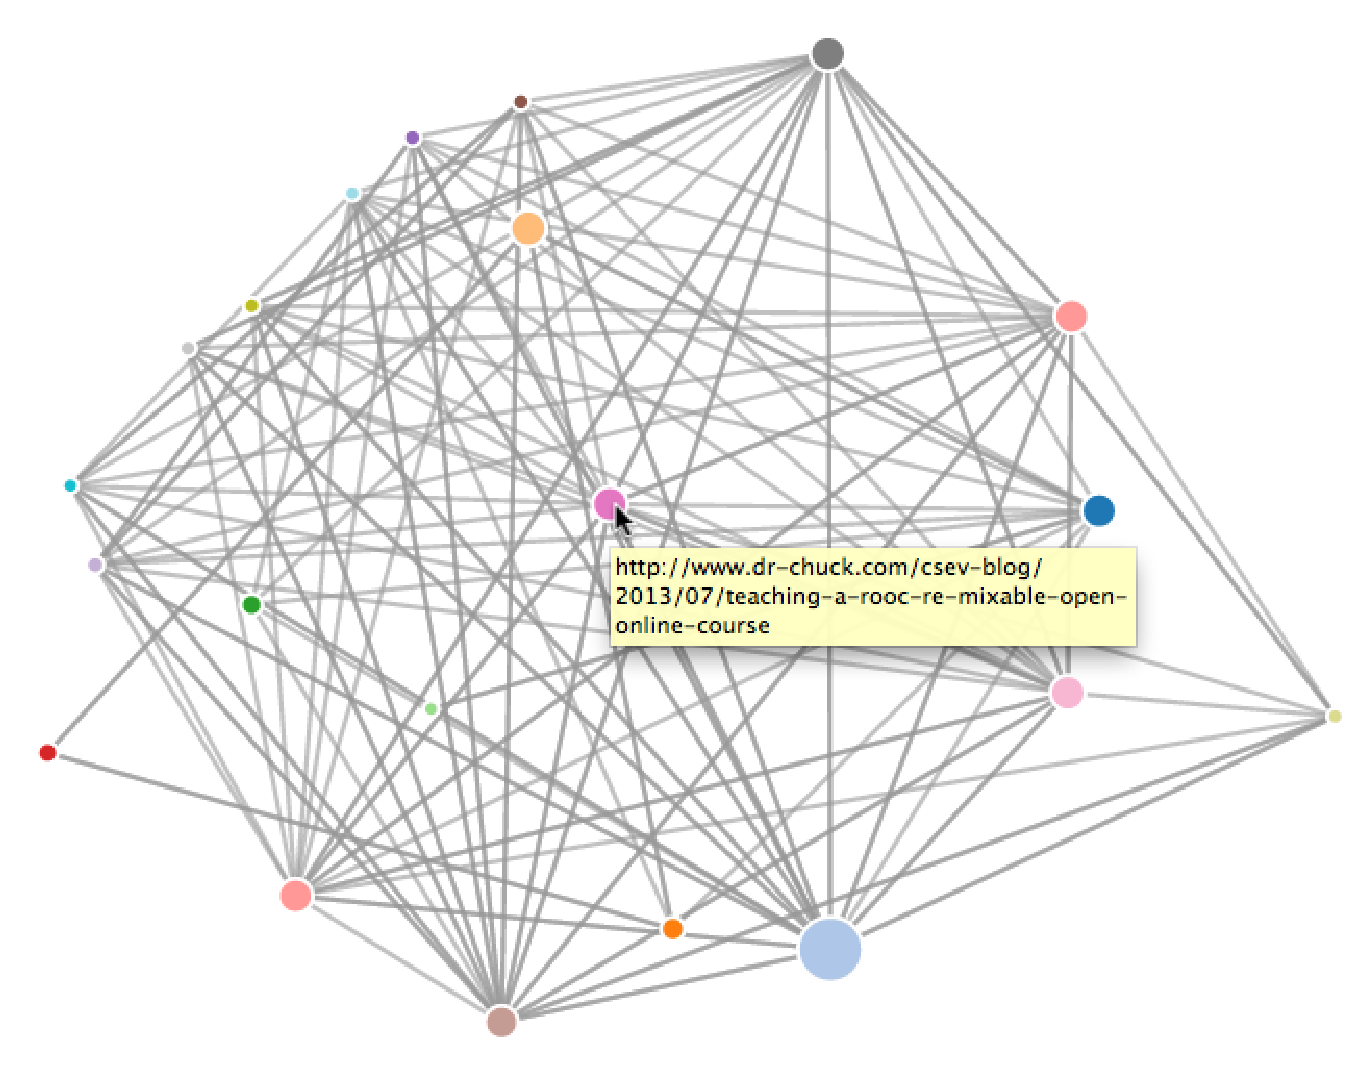
\includegraphics[height=2.25in]{figs2/pagerank.eps}}
\afterfig

O primeiro programa ({\bf spider.py}) vasculha páginas web e grava
uma série de páginas no banco de dados ({\bf spider.sqlite}), gravando
as ligações entre as páginas. Você pode reiniciar o processo a qualquer
hora deletando o arquivo {\bf spider.sqlite} e reexecutando o {\bf spider.py}.
%The first program ({\bf spider.py}) program crawls a web 
%site and pulls a series of pages into the
%database ({\bf spider.sqlite}), recording the links between pages.
%You can restart the process at any time by removing the 
%{\bf spider.sqlite} file and rerunning {\bf spider.py}.

\beforeverb
\begin{verbatim}
Enter web url or enter: http://www.dr-chuck.com/
['http://www.dr-chuck.com']
How many pages:2
1 http://www.dr-chuck.com/ 12
2 http://www.dr-chuck.com/csev-blog/ 57
How many pages:
\end{verbatim}
\afterverb
%

Neste exemplo de execução, nós pedimos ao programa para extrair e 
retornar duas páginas. Se você reiniciar o programa e pedir a ele para
obter mais páginas, não irá pegar novamente as mesmas páginas que já
estão no banco de dados. Após o restart ele vai sortear randomicamente
páginas e começar de lá. Assim, cada execução sucessiva do {\bf spider.py}
é um aditivo.
%In this sample run, we told it to crawl a website and retrieve two 
%pages.  If you restart the program and tell it to crawl more
%pages, it will not re-crawl any pages already in the database.  Upon 
%restart it goes to a random non-crawled page and starts there.  So 
%each successive run of {\bf spider.py} is additive.

\beforeverb
\begin{verbatim}
Enter web url or enter: http://www.dr-chuck.com/
['http://www.dr-chuck.com']
How many pages:3
3 http://www.dr-chuck.com/csev-blog 57
4 http://www.dr-chuck.com/dr-chuck/resume/speaking.htm 1
5 http://www.dr-chuck.com/dr-chuck/resume/index.htm 13
How many pages:
\end{verbatim}
\afterverb
%

Você pode ter múltiplos pontos de start no mesmo banco de dados, dentro
do programa, eles são chamados ``webs''. O programa escolhe randomicamente
um dos links que ainda não foi visitado através de toda a web como sendo
a próxima página a ser visitada.
%You can have multiple starting points in the same database---within
%the program, these are called ``webs''.   The spider
%chooses randomly amongst all non-visited links across all
%the webs as the next page to spider.

Se você quer visualizar o conteúdo do arquivo {\bf spider.sqlite}, você pode
rodar o programa {\bf spdump.py}, como segue:
%If you want to dump the contents of the {\bf spider.sqlite} file, you can 
%run {\bf spdump.py} as follows:

\beforeverb
\begin{verbatim}
(5, None, 1.0, 3, u'http://www.dr-chuck.com/csev-blog')
(3, None, 1.0, 4, u'http://www.dr-chuck.com/dr-chuck/resume/speaking.htm')
(1, None, 1.0, 2, u'http://www.dr-chuck.com/csev-blog/')
(1, None, 1.0, 5, u'http://www.dr-chuck.com/dr-chuck/resume/index.htm')
4 rows.
\end{verbatim}
\afterverb
%

Isto mostra o número de links visitados, o antigo page rank, o novo page
rank, o id da página, e a url da página. O programa {\bf spdump.py} somente
mostra páginas que tem pelo menos um link já visitado.
%This shows the number of incoming links, the old page rank, the new page
%rank, the id of the page, and the url of the page.  The {\bf spdump.py} program
%only shows pages that have at least one incoming link to them.

Uma vez que você tem algumas páginas no banco de dados, você pode rodar o page 
rank nas páginas usando o programa {\bf sprank.py}. Você apenas diz quantas
iterações de páginas devem ser executadas.
%Once you have a few pages in the database, you can run page rank on the
%pages using the {\bf sprank.py} program.  You simply tell it how many page
%rank iterations to run.

\beforeverb
\begin{verbatim}
How many iterations:2
1 0.546848992536
2 0.226714939664
[(1, 0.559), (2, 0.659), (3, 0.985), (4, 2.135), (5, 0.659)]
\end{verbatim}
\afterverb
%
Você pode analisar o banco de dados novamente para ver se o page rank foi
atualizado:
%You can dump the database again to see that page rank has been updated:

\beforeverb
\begin{verbatim}
(5, 1.0, 0.985, 3, u'http://www.dr-chuck.com/csev-blog')
(3, 1.0, 2.135, 4, u'http://www.dr-chuck.com/dr-chuck/resume/speaking.htm')
(1, 1.0, 0.659, 2, u'http://www.dr-chuck.com/csev-blog/')
(1, 1.0, 0.659, 5, u'http://www.dr-chuck.com/dr-chuck/resume/index.htm')
4 rows.
\end{verbatim}
\afterverb
%

Você pode rodar o {\bf sprank.py} quantas vezes quiser, isto irá apenas refinar
o page rank cada vez que você executar. Pode até mesmo rodar o {\bf sprank.py} um
pequeno número de vezes e então recuperar mais algumas páginas com o {\bf spider.py} 
e então rodar o {\bf sprank.py} para recuperar os valores do page rank. Um motor de
pesquisa geralmente roda os programas de recuperação e rankeamento ao mesmo tempo.
%You can run {\bf sprank.py} as many times as you like and it will simply refine
%the page rank each time you run it.  You can even run {\bf sprank.py} a few times
%and then go spider a few more pages sith {\bf spider.py} and then run {\bf sprank.py}
%to reconverge the page rank values.  A search engine usually runs both the crawling and 
%ranking programs all the time.

Se você quiser reiniciar os cálculos de page rank sem fazer a extração das páginas
web novamente, você pode usar o {\bf spreset.py} e então reiniciar o {\bf sprank.py}.
%If you want to restart the page rank calculations without respidering the 
%web pages, you can use {\bf spreset.py} and then restart {\bf sprank.py}.

\beforeverb
\begin{verbatim}
How many iterations:50
1 0.546848992536
2 0.226714939664
3 0.0659516187242
4 0.0244199333
5 0.0102096489546
6 0.00610244329379
...
42 0.000109076928206
43 9.91987599002e-05
44 9.02151706798e-05
45 8.20451504471e-05
46 7.46150183837e-05
47 6.7857770908e-05
48 6.17124694224e-05
49 5.61236959327e-05
50 5.10410499467e-05
[(512, 0.0296), (1, 12.79), (2, 28.93), (3, 6.808), (4, 13.46)]
\end{verbatim}
\afterverb
%

Para cada iteração do algoritmo de page rank, ele imprime a média
de modificações no page rank por página. A rede inicia-se
desbalanceada e então os valores do page rank individual mudam
com velocidade entre as iterações. Mas em poucas iterações, o page rank 
coverge. Você deve rodar o {\bf prank.py} por tempo suficiente para
que os valores de page rank possam convergir.
%For each iteration of the page rank algorithm it prints the average
%change in page rank per page.   The network initially is quite
%unbalanced and so the individual page rank values change wildly between
%iterations. But in a few short iterations, the page rank converges.  You
%should run {\bf prank.py} long enough that the page rank values converge.

Se você quer visualizar as primeiras páginas no rank, rode o {\bf spjson.py}
para ler o banco de dados e escrever os dados dos links com maior pontuação
no formato JSON para serem vistos no web browser.
%If you want to visualize the current top pages in terms of page rank,
%run {\bf spjson.py} to read the database and write the data for the 
%most highly linked pages in JSON format to be viewed in a
%web browser.

\beforeverb
\begin{verbatim}
Creating JSON output on spider.json...
How many nodes? 30
Open force.html in a browser to view the visualization
\end{verbatim}
\afterverb
%\beforeverb
%\begin{verbatim}
%Creating JSON output on spider.json...
%How many nodes? 30
%Open force.html in a browser to view the visualization
%\end{verbatim}
%\afterverb
%

Você pode visualizar este dado abrindo o arquivo {\bf force.html} em seu web 
browser. Isto mostra um layout automático de nós e links. Você pode clicar e
arrastar qualquer nó e também dar um duplo clique no nó para encontrar a URL
que ele representa.
%You can view this data by opening the file {\bf force.html} in your web browser.  
%This shows an automatic layout of the nodes and links.  You can click and 
%drag any node and you can also double-click on a node to find the URL
%that is represented by the node.

Se você rodar novamente
%If you rerun the other utilities, rerun {\bf spjson.py} and
%press refresh in the browser to get the new data from {\bf spider.json}.

\section{Visualizing mail data}

Up to this point in the book, you have become quite familiar with our 
{\bf mbox-short.txt} and {\bf mbox.txt} data files.   Now it is time to take
our analysis of email data to the next level.  

In the real world, sometimes you have to pull down mail data from servers.
That might take quite some time and the data might be inconsistent, 
error-filled, and need a lot of cleanup or adjustment.  In this section, we
work with an application that is the most complex so far and pull down nearly a 
gigabyte of data and visualize it.

\beforefig
\centerline{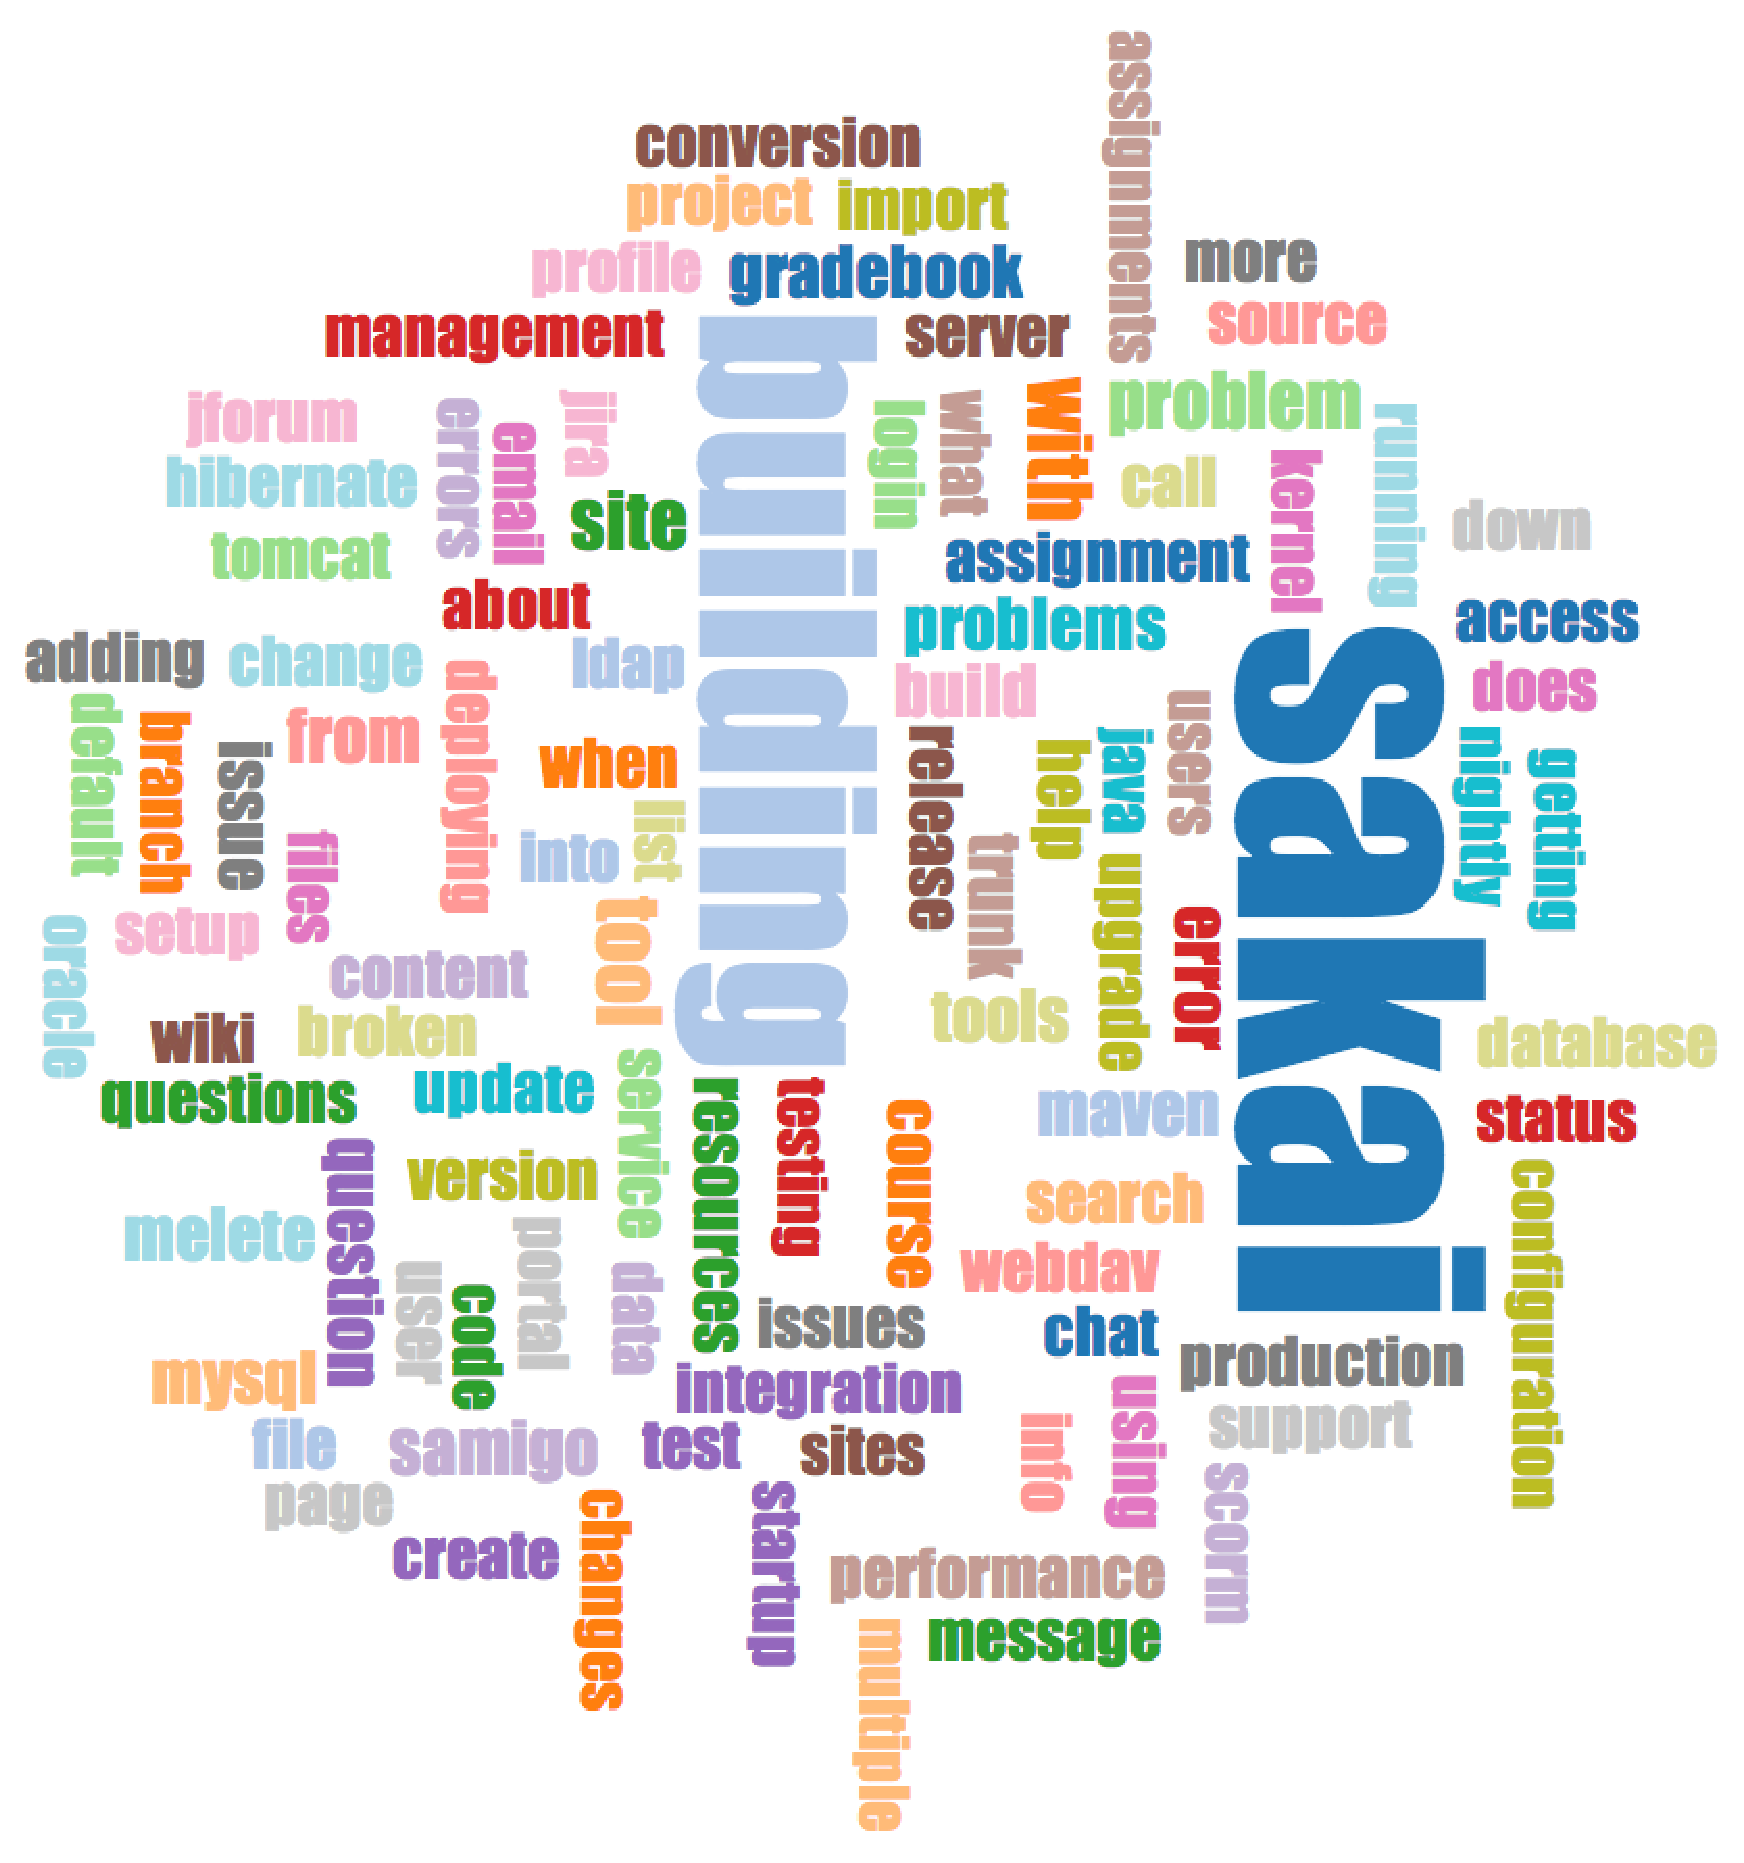
\includegraphics[height=2.50in]{figs2/wordcloud.eps}}
\afterfig

You can download this application from:

\url{www.py4inf.com/code/gmane.zip}

We will be using data from a free email list archiving service called 
\url{www.gmane.org}.  This service is very popular with open source
projects because it provides a nice searchable archive of their 
email activity.  They also have a very liberal policy regarding accessing 
their data through their API.  They have no rate limits, but ask that you 
don't overload their service and take only the data you need.  You can read
gmane's terms and conditions at this page:

\url{http://gmane.org/export.php}

{\em It is very important that you make use of the gmane.org data
responsibly by adding delays to your access of their services and spreading
long-running jobs over a longer period of time.  Do not abuse this free service
and ruin it for the rest of us.}

When the Sakai email data was spidered using this software, it produced nearly 
a Gigabyte of data and took a number of runs on several days.
The file {\bf README.txt} in the above ZIP may have instructions as to how
you can download a pre-spidered copy of the {\bf content.sqlite} file for 
a majority of the Sakai email corpus so you don't have to spider for 
five days just to run the programs.  If you download the pre-spidered
content, you should still run the spidering process to catch up with 
more recent messages.

The first step is to spider the gmane repository.  The base URL 
is hard-coded in the {\bf gmane.py} and is hard-coded to the Sakai
developer list.  You can spider another repository by changing that
base url.   Make sure to delete the {\bf content.sqlite} file if you 
switch the base url.  

The {\bf gmane.py} file operates as a responsible caching spider in 
that it runs slowly and retrieves one mail message per second so 
as to avoid getting throttled by gmane.   It stores all of
its data in a database and can be interrupted and restarted 
as often as needed.   It may take many hours to pull all the data
down.  So you may need to restart several times.

Here is a run of {\bf gmane.py} retrieving the last five messages of the
Sakai developer list:

\beforeverb
\begin{verbatim}
How many messages:10
http://download.gmane.org/gmane.comp.cms.sakai.devel/51410/51411 9460
    nealcaidin@sakaifoundation.org 2013-04-05 re: [building ...
http://download.gmane.org/gmane.comp.cms.sakai.devel/51411/51412 3379
    samuelgutierrezjimenez@gmail.com 2013-04-06 re: [building ...
http://download.gmane.org/gmane.comp.cms.sakai.devel/51412/51413 9903
    da1@vt.edu 2013-04-05 [building sakai] melete 2.9 oracle ...
http://download.gmane.org/gmane.comp.cms.sakai.devel/51413/51414 349265
    m.shedid@elraed-it.com 2013-04-07 [building sakai] ...
http://download.gmane.org/gmane.comp.cms.sakai.devel/51414/51415 3481
    samuelgutierrezjimenez@gmail.com 2013-04-07 re: ...
http://download.gmane.org/gmane.comp.cms.sakai.devel/51415/51416 0

Does not start with From 
\end{verbatim}
\afterverb
%
The program scans {\bf content.sqlite} from one up to the first message number not
already spidered and starts spidering at that message.  It continues spidering
until it has spidered the desired number of messages or it reaches a page
that does not appear to be a properly formatted message.

Sometimes \url{gmane.org} is missing a message.  Perhaps administrators can delete messages
or perhaps they get lost.   If your spider stops, and it seems it has hit
a missing message, go into the SQLite Manager and add a row with the missing id leaving
all the other fields blank and restart {\bf gmane.py}.   This will unstick the 
spidering process and allow it to continue.  These empty messages will be ignored in the next
phase of the process.

One nice thing is that once you have spidered all of the messages and have them in 
{\bf content.sqlite}, you can run {\bf gmane.py} again to get new messages as 
they are sent to the list.  

The {\bf content.sqlite} data is pretty raw, with an inefficient data model, 
and not compressed.
This is intentional as it allows you to look at {\bf content.sqlite}
in the SQLite Manager to debug problems with the spidering process.
It would be a bad idea to run any queries against this database, as they 
would be quite slow.

The second process is to run the program {\bf gmodel.py}.  This program reads the raw 
data from {\bf content.sqlite} and produces a cleaned-up and well-modeled version of the 
data in the file {\bf index.sqlite}.  This file will be much smaller (often 10X
smaller) than {\bf content.sqlite} because it also compresses the header and body text.

Each time {\bf gmodel.py} runs it deletes and rebuilds {\bf index.sqlite}, allowing
you to adjust its parameters and edit the mapping tables in {\bf content.sqlite} to tweak the 
data cleaning process. This is a sample run of {\bf gmodel.py}.  It prints a line out each time
250 mail messages are processed so you can see some progress happening, as this program may
run for a while processing nearly a Gigabyte of mail data.

\beforeverb
\begin{verbatim}
Loaded allsenders 1588 and mapping 28 dns mapping 1
1 2005-12-08T23:34:30-06:00 ggolden22@mac.com
251 2005-12-22T10:03:20-08:00 tpamsler@ucdavis.edu
501 2006-01-12T11:17:34-05:00 lance@indiana.edu
751 2006-01-24T11:13:28-08:00 vrajgopalan@ucmerced.edu
...
\end{verbatim}
\afterverb
%

The {\bf gmodel.py} program handles a number of data cleaning tasks.

Domain names are truncated to two levels for .com, .org, .edu, and .net.
Other domain names are truncated to three levels.  So si.umich.edu becomes
umich.edu and caret.cam.ac.uk becomes cam.ac.uk.   Email addresses are also
forced to lower case, and some of the @gmane.org address like the following

\beforeverb
\begin{verbatim}
   arwhyte-63aXycvo3TyHXe+LvDLADg@public.gmane.org
\end{verbatim}
\afterverb
%
are converted to the real address whenever there is a matching real email
address elsewhere in the message corpus.

In the {\bf content.sqlite} database there are two tables that allow
you to map both domain names and individual email addresses that change over 
the lifetime of the email list.  For example, Steve Githens used the following
email addresses as he changed jobs over the life of the Sakai developer list:

\beforeverb
\begin{verbatim}
s-githens@northwestern.edu
sgithens@cam.ac.uk
swgithen@mtu.edu
\end{verbatim}
\afterverb
%
We can add two entries to the Mapping table in {\bf content.sqlite} so 
{\bf gmodel.py} will map all three to one address:

\beforeverb
\begin{verbatim}
s-githens@northwestern.edu ->  swgithen@mtu.edu
sgithens@cam.ac.uk -> swgithen@mtu.edu
\end{verbatim}
\afterverb
%
You can also make similar entries in the DNSMapping table if there are multiple
DNS names you want mapped to a single DNS.  The following mapping was added to the Sakai data:

\beforeverb
\begin{verbatim}
iupui.edu -> indiana.edu
\end{verbatim}
\afterverb
%
so all the accounts from the various Indiana University campuses are tracked together.

You can rerun the {\bf gmodel.py} over and over as you look at the data, and add mappings
to make the data cleaner and cleaner.   When you are done, you will have a nicely
indexed version of the email in {\bf index.sqlite}.   This is the file to use to do data
analysis.   With this file, data analysis will be really quick.

The first, simplest data analysis is to determine "who sent the most mail?" and "which 
organization sent the most mail"?  This is done using {\bf gbasic.py}:

\beforeverb
\begin{verbatim}
How many to dump? 5
Loaded messages= 51330 subjects= 25033 senders= 1584

Top 5 Email list participants
steve.swinsburg@gmail.com 2657
azeckoski@unicon.net 1742
ieb@tfd.co.uk 1591
csev@umich.edu 1304
david.horwitz@uct.ac.za 1184

Top 5 Email list organizations
gmail.com 7339
umich.edu 6243
uct.ac.za 2451
indiana.edu 2258
unicon.net 2055
\end{verbatim}
\afterverb
%
Note how much more quickly {\bf gbasic.py} runs compared to {\bf gmane.py}
or even {\bf gmodel.py}. They are all working on the same data, but 
{\bf gbasic.py} is using the compressed and normalized data in 
{\bf index.sqlite}.  If you have a lot of data to manage, a multistep
process like the one in this application may take a little longer to develop,
but will save you a lot of time when you really start to explore
and visualize your data.

You can produce a simple visualization of the word frequency in the subject lines
in the file {\bf gword.py}:

\beforeverb
\begin{verbatim}
Range of counts: 33229 129
Output written to gword.js
\end{verbatim}
\afterverb
%

This produces the file {\bf gword.js} which you can visualize using
{\bf gword.htm} to produce a word cloud similar to the one at the beginning 
of this section.

A second visualization is produced  by {\bf gline.py}.  It computes email 
participation by organizations over time.

\beforeverb
\begin{verbatim}
Loaded messages= 51330 subjects= 25033 senders= 1584
Top 10 Oranizations
['gmail.com', 'umich.edu', 'uct.ac.za', 'indiana.edu', 
'unicon.net', 'tfd.co.uk', 'berkeley.edu', 'longsight.com', 
'stanford.edu', 'ox.ac.uk']
Output written to gline.js
\end{verbatim}
\afterverb
%
Its output is written to {\bf gline.js} which is visualized using {\bf gline.htm}.

\beforefig
\centerline{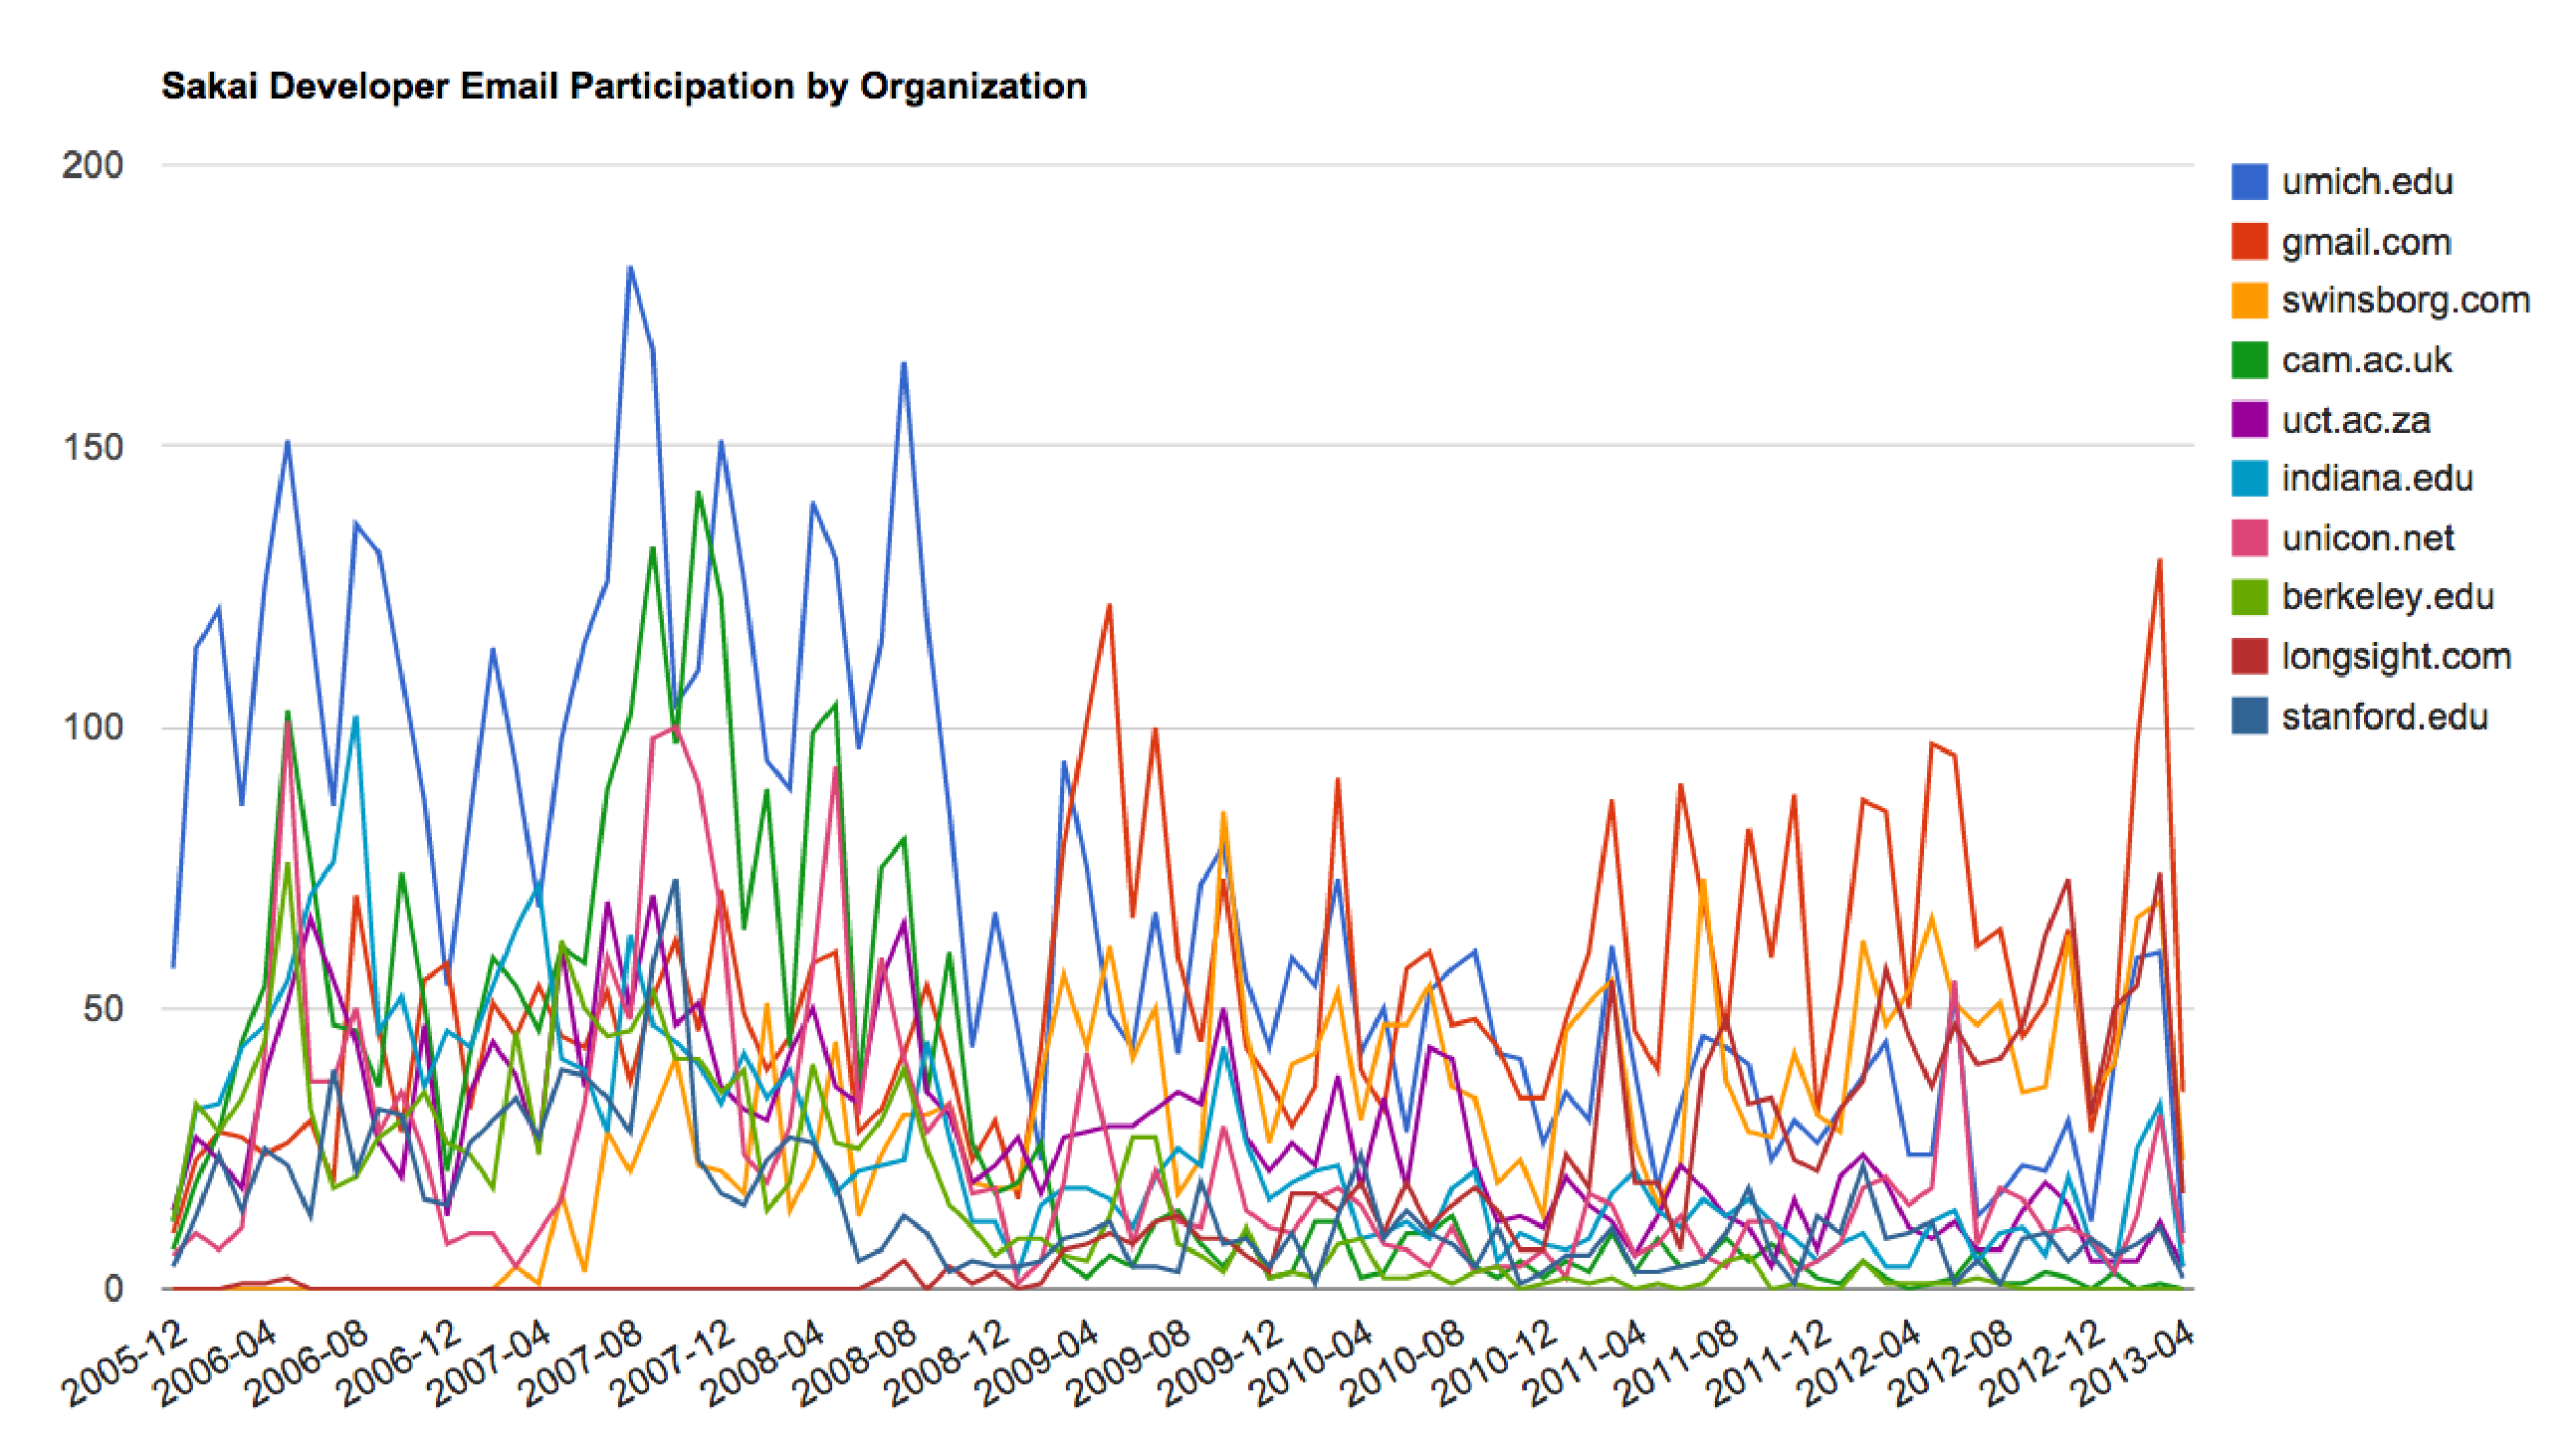
\includegraphics[height=2.50in]{figs2/mailorg.eps}}
\afterfig

This is a relatively complex and sophisticated application and 
has features to do some real data retrieval, cleaning, and visualization.
